\begin{pastexam}[label={px:gw3-108-ds-02}]{關務三等資訊處理 108 年 第二題}
（申論；30 分）

給定 T 為一個以陣列表示的二元搜尋樹（binary search tree）。
\begin{enumerate}[leftmargin=2.2em]
\item[㈠] 若有一些介於 1 及 1,000 的正整數被儲存於 T，且要搜尋數字 364，請說明搜尋過程是否有可能為 3, 400, 388,
220, 267, 383, 382, 279, 364？（5 分）
\item[㈡] 若有一些介於 1 及 1,000 的正整數被儲存於 T，且要搜尋數字 364，請說明搜尋過程是否有可能為 926, 203,
912, 241, 913, 246, 364？（5 分）
\item[㈢] 若對 T 進行前序遍歷（pre-order traversal）的結果為 30, 20, 10, 15, 25, 23, 39, 35, 42。請說明若以後序遍歷
（post-order traversal），結果為何。（5 分）
\item[㈣] 若對 T 進行後序遍歷（post-order traversal）的結果為 25, 20, 34, 37, 31, 49, 46, 57, 60, 52, 41。請說明若以
中序遍歷（in-order traversal），結果為何。（5 分）
\item[㈤] 請說明可將二元搜尋樹 T 轉換為最小堆積（min heap）的程序為何？（10 分）
\end{enumerate}
\end{pastexam}

\begin{pastsoln}
\textbf{㈠ ㈡ 的判斷方法。} 在二元搜尋樹裡找 364，每比較一個節點 $x$：$x > 364$ 就往左，之後經過的
所有數都要 $< x$；$x < 364$ 就往右，之後的都要 $> x$（資結書第~9.1~節）。 所以維護一個區間 (下界, 上界)，
每個經過的數都必須落在目前的區間內，然後依它和 364 的大小更新一邊。

\textbf{㈠ 有可能。}
\begin{center}
\begin{tabular}{cccl}
\toprule
經過 & 和 364 比 & 走向 & 之後的區間 \\
\midrule
3 & 小 & 右 & (3, 1000] \\
400 & 大 & 左 & (3, 400) \\
388 & 大 & 左 & (3, 388) \\
220 & 小 & 右 & (220, 388) \\
267 & 小 & 右 & (267, 388) \\
383 & 大 & 左 & (267, 383) \\
382 & 大 & 左 & (267, 382) \\
279 & 小 & 右 & (279, 382) \\
364 & 找到 & & \\
\bottomrule
\end{tabular}
\end{center}
每個數都落在前一步的區間內，沒有矛盾，所以這是可能的搜尋路徑。

\textbf{㈡ 不可能。} 926 大往左，區間 [1, 926)；203 小往右，(203, 926)；912 大往左，(203, 912)；
241 小往右，(241, 912)；下一個 913 必須小於 912，但 $913 > 912$，矛盾。 913 若在 912 的左子樹裡，就必須
比 912 小。 所以不可能。

\textbf{㈢ 後序：15, 10, 23, 25, 20, 35, 42, 39, 30。} 二元搜尋樹的前序第一個是根，後面比根小的那一段是左子樹、
比根大的是右子樹（資結書第~7.4~節）。 根 30；左子樹前序 20, 10, 15, 25, 23：根 20，左 10（10 的右子 15），
右 25（25 的左子 23）；右子樹前序 39, 35, 42：根 39，左 35、右 42。
\begin{center}
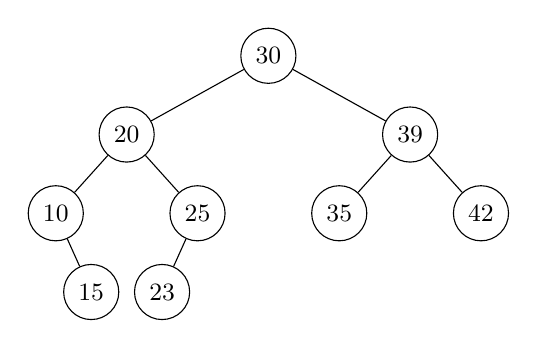
\begin{tikzpicture}[
    every node/.style={circle, draw, minimum size=7mm, inner sep=0pt, font=\small},
    level distance=10mm,
    level 1/.style={sibling distance=36mm},
    level 2/.style={sibling distance=18mm},
    level 3/.style={sibling distance=9mm}]
\node {30}
  child {node {20} child {node {10} child[missing] child {node {15}}} child {node {25} child {node {23}} child[missing]}}
  child {node {39} child {node {35}} child {node {42}}};
\end{tikzpicture}
\end{center}
後序（左、右、根）：左子樹 20 的後序是 15, 10, 23, 25, 20；右子樹 39 的後序是 35, 42, 39；最後是根 30。

\textbf{㈣ 中序：20, 25, 31, 34, 37, 41, 46, 49, 52, 57, 60。} 二元搜尋樹的中序就是鍵值由小到大（資結書
定理~9.1），所以把後序的 11 個數排序就得到答案，不必真的建樹。 檢查後序確實是合法的二元搜尋樹：最後一個
41 是根，前面 25, 20, 34, 37, 31 都 $< 41$、49, 46, 57, 60, 52 都 $> 41$，遞迴下去都切得開（樹是
41(31(20(--, 25), 37(34, --)), 52(46(--, 49), 60(57, --)))）。

\textbf{㈤ 轉換成最小堆積。} 最小堆積要求是完整二元樹、且每個節點不大於它的子節點；用陣列存時就是
$A[i] \le A[2i]$、$A[i] \le A[2i+1]$。 \textbf{由小到大排好的陣列本身就是最小堆積}：$i < 2i < 2i+1$，前面的
不會比後面的大。 二元搜尋樹的中序剛好由小到大，所以：
\begin{enumerate}
\item 對 T 做中序走訪，依序把鍵值放進新陣列 $H[1], H[2], \dots, H[n]$。
\item $H[1..n]$ 就是一個最小堆積（$H[i]$ 的子節點是 $H[2i]$、$H[2i+1]$），完成。
\end{enumerate}
\begin{pseudo}{二元搜尋樹轉最小堆積}
\Procedure{BST-To-MinHeap}{$T, H$}
    \State $k \gets 0$
    \State \Call{Inorder-Fill}{$T.\mathit{root}$} \Comment{結束時 $H[1..k]$ 就是最小堆積}
\EndProcedure
\Statex
\Procedure{Inorder-Fill}{$x$}
    \If{$x \ne \NIL$}
        \State \Call{Inorder-Fill}{$x.\mathit{left}$}
        \State $k \gets k + 1$；$H[k] \gets x.\mathit{key}$
        \State \Call{Inorder-Fill}{$x.\mathit{right}$}
    \EndIf
\EndProcedure
\end{pseudo}
中序走訪每個節點一次，時間 $\Theta(n)$。 題目的 T 是以陣列表示，若要就地轉換，也可以不管順序，直接把
T 裡的 $n$ 個鍵值緊密排到 $A[1..n]$，再做 Build-Min-Heap（從 $\lfloor n/2 \rfloor$ 往回逐一往下調整，
資結書第~8.2~節），時間也是 $\Theta(n)$。 兩種做法都對，前者利用了二元搜尋樹「中序有序」的性質，連調整都
不需要。 例如㈣ 的樹，中序 20, 25, 31, \dots, 60 依序放進陣列，就是根為 20 的最小堆積。
\end{pastsoln}
